\usetikzlibrary{positioning}
\chapter{Approaches for Neural PDE Simulators}
\label{chap:approaches}

In this chapter, we present two distinct Neural Field Turing Machine (NFTM) model architectures, developed as data-driven simulators for the 1D Burger's equation. Currently, these are defined for the simulation of Burger's dynamics and both approaches utilize the dataset described in Table~\ref{tab:dataset_Burger_statistics}, which consits of 724 training trajectories across 13 different viscosity values (from 0.001 to 0.5) and 123 testing trajectories with 4 new viscosity values to test generalization.\\
The first model \textbf{........ EXPLAIN TRANSFORMER MODEL ........}.\\
The second approach, corresponds to a \textbf{Causal Temporal Convolutional Attention Network (TCAN)} that combines attention with convolutional feature extraction, by restricting attention to past timesteps only and using 1D convolutions for spatial processing.\\
Both approaches enforce physics-informed constraints. We detail their architectures, training procedures, and comprehensive evaluation metrics, highlighting respective strengths and limitations.

% TABLE OF BURGER'S DATASET STATISTICS
\begin{table}[htbp]
\centering
\caption{Burger's Equation Dataset: Number of Trajectories by Viscosity.}
\label{tab:dataset_Burger_statistics}
\resizebox{0.75\textwidth}{!}{
\begin{tabular}{c c c c}
\toprule
\multicolumn{4}{c}{\textbf{Training (724 samples)}} \\
\midrule
\textbf{Viscosity $\nu$} & \textbf{Count} & \textbf{Percentage} & \\
\midrule
0.0010 & 60 & 8.3\% & \\
0.0020 & 40 & 5.5\% & \\
0.0065 & 40 & 5.5\% & \\
0.0080 & 40 & 5.5\% & \\
0.0400 & 40 & 5.5\% & \\
0.0500 & 60 & 8.3\% & \\
0.0700 & 60 & 8.3\% & \\
0.1000 & 60 & 8.3\% & \\
0.1500 & 60 & 8.3\% & \\
0.2500 & 60 & 8.3\% & \\
0.3500 & 60 & 8.3\% & \\
0.4000 & 60 & 8.3\% & \\
0.5000 & 84 & 11.6\% & \\
\midrule
\multicolumn{4}{c}{\textbf{Testing (123 samples)}} \\
\midrule
0.0100 & 50 & 40.7\% & \\
0.0269 & 13 & 10.6\% & \\
0.2000 & 30 & 24.4\% & \\
0.3000 & 30 & 24.4\% & \\
\bottomrule
\end{tabular}
}
\end{table}

% ----------------------------------------------------------- SAMUEL MODEL -------------------------------------------------------------------------------
\section{Approach 1: Transformer based Model}
\subsection{Model Architecture}
\subsection{}


% ----------------------------------------------------------- AKASH MODEL -------------------------------------------------------------------------------
\section{Approach 2: TCAN based Model}
\subsection{Model Architecture}
The Temporal Convolutional Attention Network (TCAN) is a feed-forward autoregressive model that predicts next state of a PDE given a sliding window of past states.
The TCAN serves as the \textit{controller} in the Neural Field Turing Machine model framework, where it learns a discrete-time update rule for continuous spatiotemporal fields.\\
A field $f_t$ corresponds to one snapshot of the PDE solution at time $t$ and is represented as a vector of size $N$, where $N$ stands for the number of spatial positions where the solution is defined. Therefore, the continuous field at time $t$ is given by: $$f_t = [u(x_1, t), u(x_2, t),..., u(x_N,t)] \in \mathbb{R}^{1 \times N}.$$
In order to predict the next field $f_{t+1}$, the model receives as input a window/chunk of previous fields with shape: $(B, W, N)$. This is defined as: $$\text{window} = [f_{t - W + 1}, f_{t - W + 2}, ..., f_{t}],$$ where $B$ is the batch size, $W$ is the history length (number of previous fields in the window), and $N$ is the number of spatial points.\\
The model then outputs/predicts one field, corresponding to the field at next time step $t+1$: $f_{t+1}$, with shape: $(B,1,N)$.\\\\
Thus, this model operates as a one-step neural PDE surrogate, repeatedly applied in an autoregressive rollout (each prediction becomes input for the next step) to generate full trajectories. Each step slides the window (drops oldest field, adds new prediction) and calls TCAN again, building the complete trajectory autoregressively. Figure~\ref{fig:autoregressive-rollout} illustrates this process.
\vspace{0.3cm}
\begin{figure}[htbp]
\centering
\resizebox{0.5\textwidth}{!}{%
\begin{tikzpicture}[
    box/.style={draw, rectangle, rounded corners, minimum width=2.2cm, minimum height=0.8cm, align=center, fill=orange!20, font=\small},
    pred/.style={draw, rectangle, rounded corners, minimum width=1.6cm, minimum height=0.8cm, align=center, fill=green!20, font=\small},
    arrow/.style={->, thick, >=stealth},
    node distance=1.4cm
]

% Step 1
\node[box] (w1) {Window\\$[f_1,\dots,f_{20}]$};
\node[pred, right=of w1] (p21) {$\hat{f}_{21}$};
\node[font=\scriptsize, above=0.10cm of $(w1)!0.52!(p21)$] {TCAN};
\draw[arrow] (w1.east) -- (p21.west);

% Step 2
\node[box, below=of w1] (w2) {Window\\$[f_2,\dots,f_{20},f_{21}]$};
\node[pred, right=of w2] (p22) {$\hat{f}_{22}$};
\node[font=\scriptsize, above=-0.55cm of $(w2)!0.55!(p22)$] {TCAN};
\draw[arrow] (w2.east) -- (p22.west);

% Step 3
\node[box, below=of w2] (w3) {Window\\$[f_3,\dots,f_{21},f_{22}]$};
\node[pred, right=of w3] (p23) {$\hat{f}_{23}$};
\node[font=\scriptsize, above=-0.45cm of $(w3)!0.55!(p23)$] {TCAN};
\draw[arrow] (w3.east) -- (p23.west);

% Pred → next window (curvas por debajo, lejos del texto TCAN)
\draw[arrow] (p21.south) to[out=-60,in=20] (w2.north);
\draw[arrow] (p22.south) to[out=-60,in=20] (w3.north);


% Continuation dots
\node[font=\large] (dots) at ($(w3.south)!0.5!(p23.south) + (0,-1.2)$) {$\dots$};

\end{tikzpicture}%
}
\vspace{0.4cm}
\caption{Autoregressive rollout process: each TCAN call maps a window of previous fields to one predicted field. The prediction is inserted into the next window, replacing the oldest field, to generate the full trajectory. In this example, the model first predicts $f_{21}$ from the window $[f_1,\dots,f_{20}]$, then uses the updated window $[f_2,\dots,f_{20},f_{21}]$ to predict $f_{22}$, and so on.}
\label{fig:autoregressive-rollout}
\end{figure}

\noindent The architecture of this TCAN model consists of \textbf{three main components}:\\
\textbf{1.} A temporal attention encoder that aggregates information across the history window.\\
\textbf{2.} A convolutional decoder that produces a bounded correction.\\
\textbf{3.} A residual update that adds the correction to the last frame.\\\\
The full data flow for a single prediction step is illustrated in Figure~\ref{fig:tcn-flow}.

\begin{figure}[htbp]
\centering
\resizebox{0.95\textwidth}{!}{%
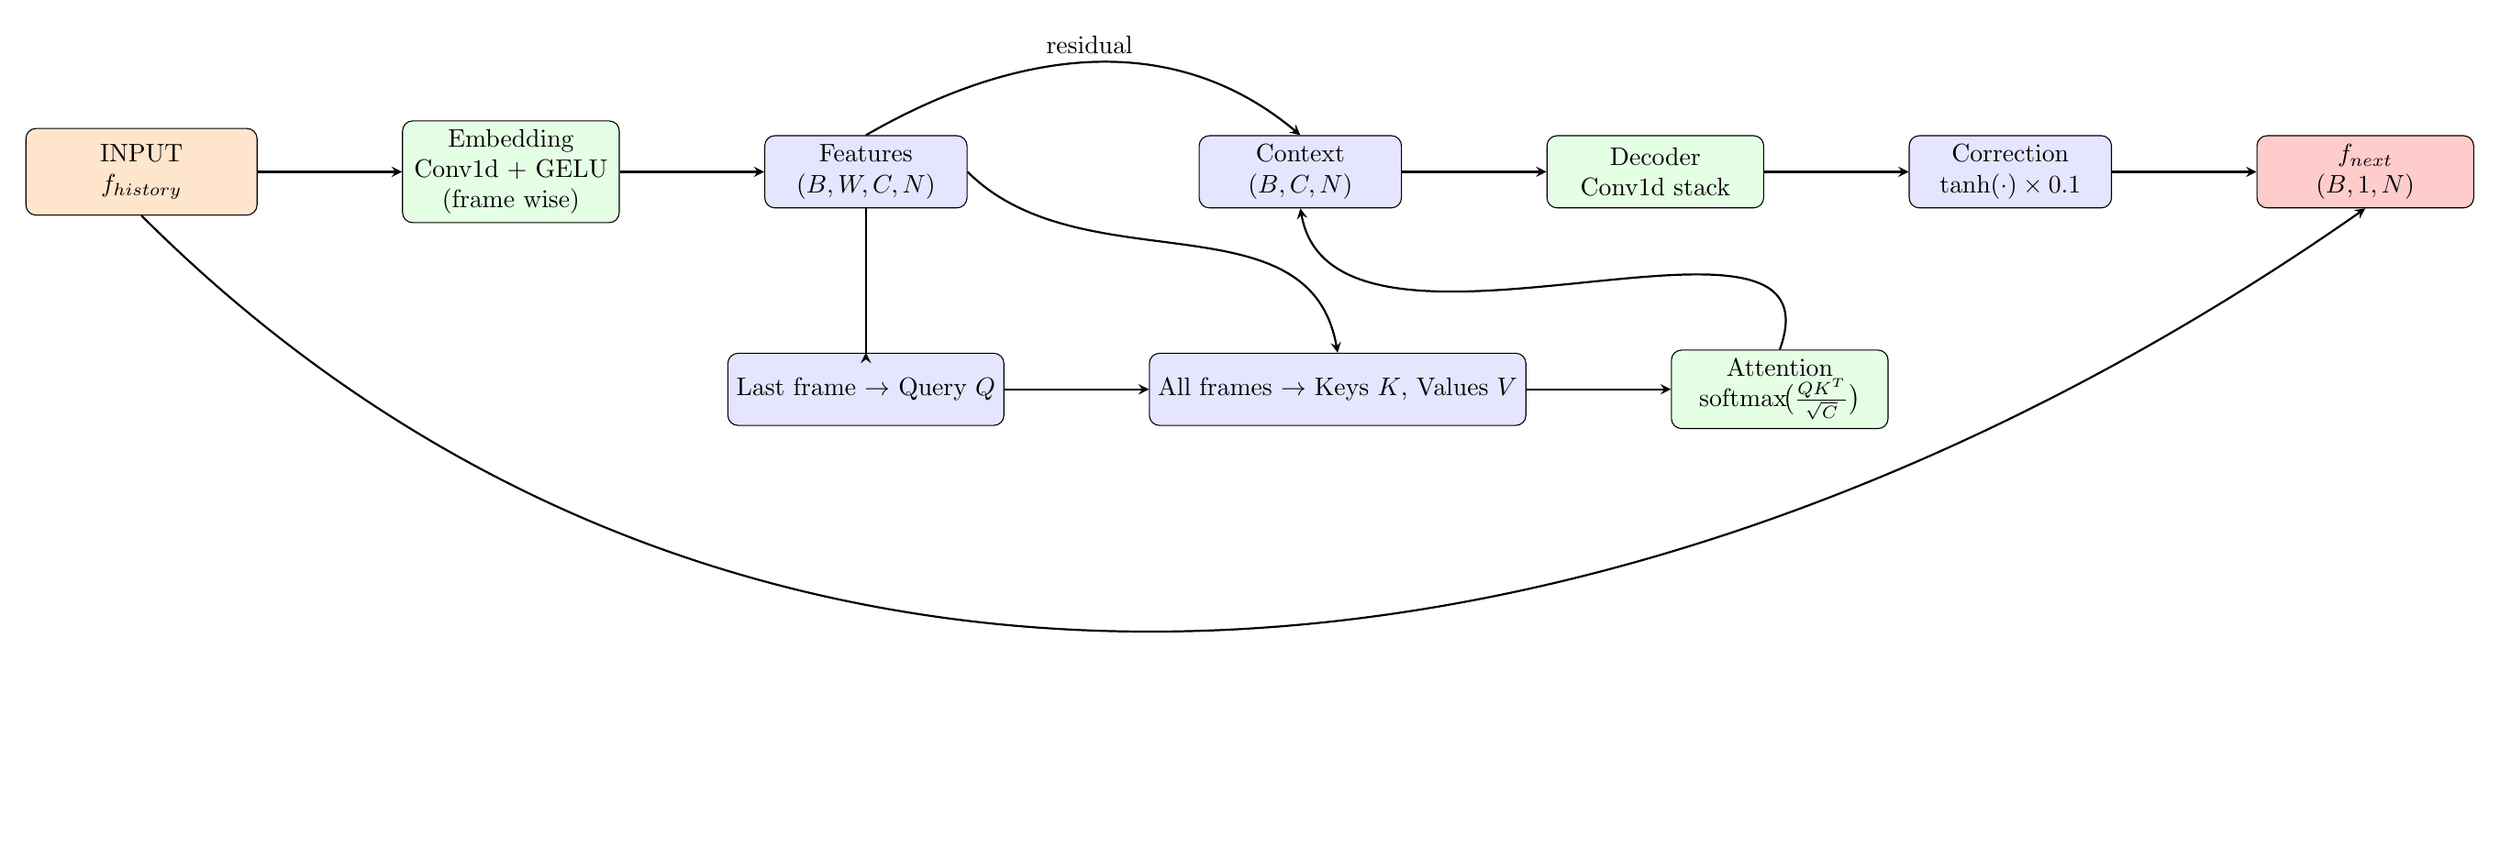
\begin{tikzpicture}[
    box/.style={rectangle, draw, rounded corners, minimum width=2.8cm, minimum height=1cm, align=center, fill=blue!10},
    op/.style={rectangle, draw, rounded corners, minimum width=3cm, minimum height=1cm, align=center, fill=green!10},
    arrow/.style={->, thick, >=stealth},
    input/.style={rectangle, draw, rounded corners, minimum width=3.2cm, minimum height=1.2cm, align=center, fill=orange!20},
    output/.style={rectangle, draw, rounded corners, minimum width=3cm, minimum height=1cm, align=center, fill=red!20},
    node distance=2.0cm
]

% Fila superior: flujo principal
\node[input] (input) {INPUT\\$f_{\text{history}}$};
\node[op, right=of input] (embed) {Embedding \\ Conv1d + GELU\\(frame wise)};
\node[box, right=of embed] (features) {Features\\$(B, W, C, N)$};
\node[box, right=3.2cm of features] (context) {Context\\$(B, C, N)$};
\node[op, right=of context] (decoder) {Decoder\\Conv1d stack};
\node[box, right=of decoder] (corr) {Correction\\$\tanh(\cdot)\times 0.1$};
\node[output, right=of corr] (output) {$f_{\text{next}}$\\$(B, 1, N)$};

% Fila inferior: atención temporal
\node[box, below=2.0cm of features] (query) {Last frame $\rightarrow$ Query $Q$};
\node[box, right=of query] (kv) {All frames $\rightarrow$ Keys $K$, Values $V$};
\node[op, right=of kv] (attn) {Attention\\$\mathrm{softmax}\!\big(\frac{QK^{T}}{\sqrt{C}}\big)$};

% Flechas flujo principal (superior)
\draw[arrow] (input) -- (embed);
\draw[arrow] (embed) -- (features);
\draw[arrow] (context) -- (decoder);
\draw[arrow] (decoder) -- (corr);
\draw[arrow] (corr) -- (output);

% Flecha a Query: igual que antes
\draw[arrow] (features.south) |- (query.north);

% Flecha a Keys/Values: menos baja, gira antes a la derecha
\draw[arrow] (features.east) to[out=-45,in=100] (kv.north);

% Flechas dentro de la rama de atención
\draw[arrow] (query) -- (kv);
\draw[arrow] (kv) -- (attn);

% De atención a contexto: giro bajo
\draw[arrow] (attn.north) to[out=70,in=-80] (context.south);

% Residual de features a context (por arriba)
\draw[arrow] (features.north) to[out=30,in=140] node[above]{residual} (context.north);

% Residual de u_history a u_next (sin texto, menos alto)
\draw[arrow] (input.south) to[out=-45,in=-145] (output.south);

\end{tikzpicture}%
}
\caption{Data flow through the Causal Temporal Attention Network during one prediction step.}
\label{fig:tcn-flow}
\end{figure}

\noindent Figure~\ref{fig:tcn-flow} illustrates the complete data flow through the Causal Temporal Convolutional Attention Network during a single prediction step. Each node performs a specific transformation:

\begin{itemize}
    \item \textbf{$f_{\text{history}}$ (Input)}: Window of $W=20$ previous fields of shape $(B, W, N)$, containing the most recent spatiotemporal snapshots $f_{t-W+1}, \dots, f_t \in \mathbb{R}^N$.
    
    \item \textbf{Conv1d + GELU (frame-wise)}: Applies 1D convolution (kernel size 3) to each of the $W$ fields individually, expanding from 1 to $C=32$ feature channels per field. Output shape: $(B \cdot W, 32, N)$.
    
    \item \textbf{Features $(B, W, C, N)$}: Reshaped embedded representation exposing the temporal dimension, with each of the $W$ fields now containing 32 spatial feature maps.
    
    \item \textbf{Last frame $\to$ Query $Q$}: Extracts features from the most recent field $f_t$ and applies $1\times1$ convolution to generate query vectors $Q \in \mathbb{R}^{B \times 32 \times N}$.
    
    \item \textbf{All frames $\to$ Keys $K$, Values $V$}: Projects all $W$ embedded fields through separate $1\times1$ convolutions to produce keys $K$ and values $V$, both of shape $(B, W, 32, N)$.
    
    \item \textbf{Attention $\mathrm{softmax}\big(\frac{QK^{T}}{\sqrt{C}}\big)$}: Computes causal attention scores between the query (last frame) and all previous frames, producing temporal attention weights $\alpha_{w,p} = \mathrm{softmax}_w(QK^T/\sqrt{32})$ for each spatial position $p$.
    
    \item \textbf{Context $(B, C, N)$}: Aggregates temporal context via weighted sum $\sum_w \alpha_{w,p} V_w$, adds residual connection from last-frame features, and applies GroupNorm. Shape: $(B, 32, N)$.
    
    \item \textbf{Decoder Conv1d stack}: Two-layer convolutional decoder (32$\to$32$\to$1 channels, kernel size 5) that maps rich temporal-spatial context to a scalar correction field. Final layer zero-initialized for training stability.
    
    \item \textbf{Correction $\tanh(\cdot)\times 0.1$}: Applies hyperbolic tangent nonlinearity scaled by 0.1 to bound corrections $|\Delta u| \leq 0.1$, ensuring numerical stability during long rollouts.
    
    \item \textbf{$u_{\text{next}}$ (Output)}: Residual update combining the last input field $u_{\text{history}}[:, -1, :]$ with the predicted correction: $f_{t+1} = f_t + \Delta u$. Shape: $(B, 1, N)$.
\end{itemize}

The two residual connections---from Features to Context (within attention encoder) and from input last frame to output---preserve critical spatiotemporal information while enabling stable incremental updates.




\subsection{Temporal Attention Encoder}

The \texttt{CausalTemporalAttention} module processes the history window through the following steps:

\begin{enumerate}
    \item \textbf{Frame-wise embedding}: Reshape $u_{\text{history}}$ to $(B \cdot W, 1, P)$ and apply a 1D convolution with kernel size 3 followed by GELU activation, producing features of shape $(B \cdot W, C, P)$ where $C=32$ is the embedding dimension.
    
    \item \textbf{Temporal restructuring}: Reshape features back to $(B, W, C, P)$ to expose the temporal dimension.
    
    \item \textbf{Query computation}: Extract features of the last frame $\text{features}[:, -1, :, :] \in \mathbb{R}^{B \times C \times P}$ and apply a $1 \times 1$ convolution to obtain queries $Q \in \mathbb{R}^{B \times C \times P}$.
    
    \item \textbf{Key and value projection}: Apply $1 \times 1$ convolutions to all $W$ frames (flattened to $(B \cdot W, C, P)$ then reshaped) to obtain keys $K$ and values $V$, both of shape $(B, W, C, P)$.
    
    \item \textbf{Causal attention scores}: Compute scaled dot-product attention over the temporal dimension:
    \[
    \text{scores}_{b,w,p} = \frac{\langle Q_b, K_{b,w} \rangle}{\sqrt{C}}, \quad \alpha_{b,w,p} = \text{softmax}_w(\text{scores}_{b,w,p})
    \]
    
    \item \textbf{Context aggregation}: Compute the attended context:
    \[
    \text{context}_b = \sum_{w=1}^W \alpha_{b,w} \cdot V_{b,w} \in \mathbb{R}^{B \times C \times P}
    \]
    
    \item \textbf{Residual projection}: Apply a $1 \times 1$ convolution to the context, add the residual connection to the last frame features, and normalize with GroupNorm.
\end{enumerate}

This mechanism allows the last frame to dynamically query relevant past frames at each spatial location, producing spatially-aware temporal context features.

\subsection{Decoder and Residual Correction}

The \texttt{ImprovedBurgersNet} decoder processes the attention output $\text{context} \in \mathbb{R}^{B \times C \times P}$ as follows:

\begin{enumerate}
    \item \textbf{Convolutional decoder stack}:
    \begin{itemize}
        \item Conv1d: $C \to 32$ channels, kernel size 5, BatchNorm1d, GELU.
        \item Conv1d: $32 \to 1$ channel, kernel size 5, producing $\text{raw\_correction} \in \mathbb{R}^{B \times 1 \times P}$.
    \end{itemize}
    The final layer is zero-initialized to ensure near-zero corrections during early training.
    
    \item \textbf{Bounded correction}: Apply hyperbolic tangent clipping scaled by $\text{corr\_clip}=0.1$:
    \[
    \Delta u = \tanh(\text{raw\_correction}) \cdot 0.1
    \]
    
    \item \textbf{Residual update}: Add the correction to the last input frame:
    \[
    u_{\text{next}} = u_{\text{history}}[:, -1:, :] + \Delta u
    \]
\end{enumerate}

This design enforces incremental updates, preventing instability during long autoregressive rollouts.

\subsection{Autoregressive Training Procedure}

Training employs curriculum learning with multi-step rollouts:

\begin{enumerate}
    \item Initialize $\text{current\_window} = u_{\text{gt}}[:, :W, :]$ from ground truth trajectories.
    
    \item For each rollout step $k \in \{0, \dots, D-1\}$ where $D$ is the rollout depth (curriculum: 8$\to$16$\to$64):
    \begin{itemize}
        \item Predict $\hat{u}_{W+k} = \text{TCAN}(\text{current\_window})$.
        \item Compute composite loss:
        \[
        \mathcal{L} = \text{MSE}(\hat{u}, u_{\text{gt}}) + 0.1 \cdot \|\nabla_x \hat{u} - \nabla_x u_{\text{gt}}\|_2^2 + 0.05 \cdot \mathbb{E}[\max(0, E(\hat{u}) - E(u_t))]
        \]
        where $E(u) = \frac{1}{2} \int u^2 \, dx$ enforces energy dissipation.
        \item Update window: $\text{current\_window} \gets [\text{current\_window}[:, 1:, :], \hat{u}]$ (with occasional teacher forcing).
    \end{itemize}
    
    \item Average loss over rollout, backpropagate through unrolled computation graph, apply gradient clipping, and optimize with AdamW + cosine annealing.
\end{enumerate}

\subsection{Evaluation Metrics}

Full-trajectory predictions are evaluated using:
\begin{itemize}
    \item Standard: MSE, relative $L^2$, PSNR, SSIM, temporal correlation.
    \item Physics-informed: mass conservation error, energy monotonicity fraction, mean PDE residual, spectral error, max gradient error.
\end{itemize}

This comprehensive evaluation ensures both accuracy and physical fidelity across long rollouts.
